\section{Force estimation}\label{sec:force_estimation}
In order to have a representation of the reaction force on the EndoWrist, estimation is needed.
Because of the reasons mentioned in Section \ref{sec:system_overview}, the force cannot be measured using sensors and thus have to rely on mathematical models as functions of torque measurements.

\subsection{Mathematical model}
The main challenge faced in making a model lies in the fact that the pulley system on the EndoWrist is nonlinear, and thus its full dynamics cannot be modeled in a straightforward manner. 
The nonlinearity of EndoWrist dynamics emerges from friction and elasticity of the pulley strings controlling the end-effector, which causes multiple pulleys to move as a result of actuating only one. 
In other words, to have an accurate representation of Cartesian force a higher order nonlinear model is required.

Another method of tackling this problem lies in creating multiple mathematical models pertaining to forces output by actions performed with the EndoWrist.
In this manner, the feedback vector is transformed from Cartesian space to a task space in which the chosen actions form a basis.
Each element of the new feedback vector corresponds to an actuated axis of the Geomagic Touch.
For the purpose of this system, we choose to feedback the yaw force generated by the grip action of the clamp, the force generated by the roll actuator and force exerted by the clamps pitch movement, as seen in \ref{fig:endowrits_set}.

\subsection{System Identification}
Ideally, a mathematical model derived from classical mechanics would be used to describe the dynamics involved in EndoWrist movement.
However, deriving this model precisely enough for grey-box identification has been proven difficult and time consuming due to the nonlinear nature of the dynamics \cite{kim2014dynamic}.

Models for yaw and pitch forces require the utilization of so called black-box identification algorithms, which only provide a general model structure. 
A straightforward approach would involve choosing a nonlinear model structure for identification.
On the other hand, stability analysis of nonlinear models is difficult and due to the nature of the system only general trends in force need to be represented.
For this reason it was decided to identify a linear state-space model which is then used as a part of Hammerstein-Wiener  \cite{zhu2002estimation} nonlinear model as seen in Fig. \ref{fig:weiner}.


\begin{figure}[h] 
\resizebox{\columnwidth}{!}{
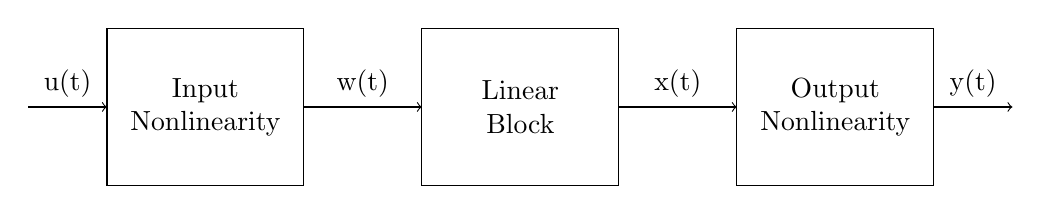
\begin{tikzpicture}%[scale=0.85]
\draw  (-7,3) rectangle (-4.5,1) node[pos=.5,align=center] {Input\\Nonlinearity};
\draw  (-3,3) rectangle (-0.5,1) node[pos=.5,align=center] {Linear\\Block};%
\draw  (1,3) rectangle (3.5,1) node[pos=.5,align=center] {Output\\Nonlinearity};

\draw [->] (-4.5,2) -- (-3,2) node [pos=0.5,above] {w(t)};
\draw [->] (-8,2) -- (-7,2) node [pos=0.5,above] {u(t)};
\draw [->] (-0.5,2) -- (1,2) node [pos=0.5,above] {x(t)};
\draw [->] (3.5,2) -- (4.5,2) node [pos=0.5,above] {y(t)};
\end{tikzpicture}
}
\caption{Block diagram of a Hammerstein-Wiener model.}
\label{fig:weiner}
\end{figure}

\subsubsection{Roll force}
The roll force, which is determined by the roll actuator and directly rotates the entire tool, making it independent to the rest of the system.
By simple measurement with the setup as seen in (SETUP PICTURE) we can interpret the roll force as determined by a feedthrough component in the state space model of the system.



\begin{equation}
\resizebox{0.91\hsize}{!}{
$\mathbf{x}(k+1) = 
\begin{bmatrix} \mathbf{0} & \mathbf{0} & \mathbf{0}\\
\mathbf{0} & \mathbf{A}_{pitch} &\mathbf{0}\\
\mathbf{0} &\mathbf{0} & \mathbf{A}_{yaw}  \end{bmatrix} 
\mathbf{x}(k) + 
\begin{bmatrix} \mathbf{B}_{roll} & \mathbf{0} & \mathbf{0}\\
\mathbf{0} & \mathbf{B}_{pitch} &\mathbf{0}\\
\mathbf{0} &\mathbf{0} & \mathbf{B}_{yaw}  \end{bmatrix} 
\mathbf{u}(k)$
}
\end{equation}

\begin{equation}\label{eq:allSS}
\resizebox{0.5\hsize}{!}{
	$\mathbf{y}(k+1) = 
	\begin{bmatrix} \mathbf{C}_{roll} & \mathbf{0} & \mathbf{0}\\
	\mathbf{0} & \mathbf{C}_{pitch} &\mathbf{0}\\
	\mathbf{0} &\mathbf{0} & \mathbf{C}_{yaw}  \end{bmatrix} 
	\mathbf{x}(k) $}
\end{equation}

\subsubsection{Pitch and yaw forces}
The pitch and yaw force state space models were determined using subspace identification  \cite{van2012subspace}. This algorithm combines concepts from system theory, linear algebra and statistics in order to provide a state-space model of the system, which makes it useful for MIMO system identification. 

Actuator effort and velocity were used as inputs during identification.
The order of identified model was picked using singular value analysis, which determines the amount of data dynamics a model can describe at a given order. For both the pitch and yaw forces, it was determined that 6th order models are sufficient. 

Deadzone nonlinearities were estimated for the inputs and output of the models. The resulting Hammerstein-Wiener models were validated on previously unused data.

%  \begin{figure}[H]
%  \centering
% 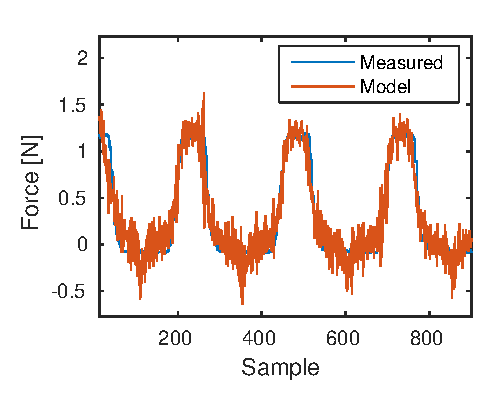
\includegraphics[width=0.49\linewidth]{modelpitch2_a}
% 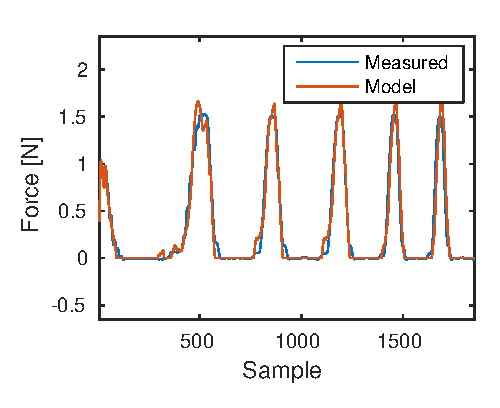
\includegraphics[width=0.49\linewidth]{modelyaw_a}
% \caption{Comparison of pitch (left) and yaw (right) model to measurements.}
% \label{fig:final_res_yaw}
% \end{figure}

%  \begin{figure}[H]
%  \centering
% 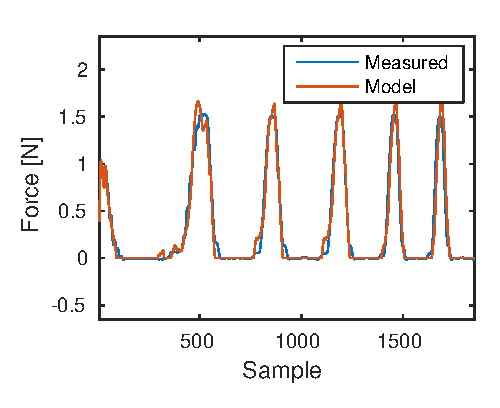
\includegraphics[width=\linewidth]{modelyaw_a}
% \caption{Comparison of yaw model to measurements.}
% \label{fig:final_res_yaw}
% \end{figure}


